\documentclass[]{article}
\usepackage{lmodern}
\usepackage{amssymb,amsmath}
\usepackage{ifxetex,ifluatex}
\usepackage{fixltx2e} % provides \textsubscript
\ifnum 0\ifxetex 1\fi\ifluatex 1\fi=0 % if pdftex
  \usepackage[T1]{fontenc}
  \usepackage[utf8]{inputenc}
\else % if luatex or xelatex
  \ifxetex
    \usepackage{mathspec}
  \else
    \usepackage{fontspec}
  \fi
  \defaultfontfeatures{Ligatures=TeX,Scale=MatchLowercase}
\fi
% use upquote if available, for straight quotes in verbatim environments
\IfFileExists{upquote.sty}{\usepackage{upquote}}{}
% use microtype if available
\IfFileExists{microtype.sty}{%
\usepackage{microtype}
\UseMicrotypeSet[protrusion]{basicmath} % disable protrusion for tt fonts
}{}
\usepackage[margin=1in]{geometry}
\usepackage{hyperref}
\PassOptionsToPackage{usenames,dvipsnames}{color} % color is loaded by hyperref
\hypersetup{unicode=true,
            pdftitle={Learning Genetic and Environmental Graphical Models using the R package FamilyBasedPGMs},
            pdfauthor={Adèle Helena Ribeiro},
            colorlinks=true,
            linkcolor=Maroon,
            citecolor=Blue,
            urlcolor=blue,
            breaklinks=true}
\urlstyle{same}  % don't use monospace font for urls
\usepackage{color}
\usepackage{fancyvrb}
\newcommand{\VerbBar}{|}
\newcommand{\VERB}{\Verb[commandchars=\\\{\}]}
\DefineVerbatimEnvironment{Highlighting}{Verbatim}{commandchars=\\\{\}}
% Add ',fontsize=\small' for more characters per line
\usepackage{framed}
\definecolor{shadecolor}{RGB}{248,248,248}
\newenvironment{Shaded}{\begin{snugshade}}{\end{snugshade}}
\newcommand{\KeywordTok}[1]{\textcolor[rgb]{0.13,0.29,0.53}{\textbf{#1}}}
\newcommand{\DataTypeTok}[1]{\textcolor[rgb]{0.13,0.29,0.53}{#1}}
\newcommand{\DecValTok}[1]{\textcolor[rgb]{0.00,0.00,0.81}{#1}}
\newcommand{\BaseNTok}[1]{\textcolor[rgb]{0.00,0.00,0.81}{#1}}
\newcommand{\FloatTok}[1]{\textcolor[rgb]{0.00,0.00,0.81}{#1}}
\newcommand{\ConstantTok}[1]{\textcolor[rgb]{0.00,0.00,0.00}{#1}}
\newcommand{\CharTok}[1]{\textcolor[rgb]{0.31,0.60,0.02}{#1}}
\newcommand{\SpecialCharTok}[1]{\textcolor[rgb]{0.00,0.00,0.00}{#1}}
\newcommand{\StringTok}[1]{\textcolor[rgb]{0.31,0.60,0.02}{#1}}
\newcommand{\VerbatimStringTok}[1]{\textcolor[rgb]{0.31,0.60,0.02}{#1}}
\newcommand{\SpecialStringTok}[1]{\textcolor[rgb]{0.31,0.60,0.02}{#1}}
\newcommand{\ImportTok}[1]{#1}
\newcommand{\CommentTok}[1]{\textcolor[rgb]{0.56,0.35,0.01}{\textit{#1}}}
\newcommand{\DocumentationTok}[1]{\textcolor[rgb]{0.56,0.35,0.01}{\textbf{\textit{#1}}}}
\newcommand{\AnnotationTok}[1]{\textcolor[rgb]{0.56,0.35,0.01}{\textbf{\textit{#1}}}}
\newcommand{\CommentVarTok}[1]{\textcolor[rgb]{0.56,0.35,0.01}{\textbf{\textit{#1}}}}
\newcommand{\OtherTok}[1]{\textcolor[rgb]{0.56,0.35,0.01}{#1}}
\newcommand{\FunctionTok}[1]{\textcolor[rgb]{0.00,0.00,0.00}{#1}}
\newcommand{\VariableTok}[1]{\textcolor[rgb]{0.00,0.00,0.00}{#1}}
\newcommand{\ControlFlowTok}[1]{\textcolor[rgb]{0.13,0.29,0.53}{\textbf{#1}}}
\newcommand{\OperatorTok}[1]{\textcolor[rgb]{0.81,0.36,0.00}{\textbf{#1}}}
\newcommand{\BuiltInTok}[1]{#1}
\newcommand{\ExtensionTok}[1]{#1}
\newcommand{\PreprocessorTok}[1]{\textcolor[rgb]{0.56,0.35,0.01}{\textit{#1}}}
\newcommand{\AttributeTok}[1]{\textcolor[rgb]{0.77,0.63,0.00}{#1}}
\newcommand{\RegionMarkerTok}[1]{#1}
\newcommand{\InformationTok}[1]{\textcolor[rgb]{0.56,0.35,0.01}{\textbf{\textit{#1}}}}
\newcommand{\WarningTok}[1]{\textcolor[rgb]{0.56,0.35,0.01}{\textbf{\textit{#1}}}}
\newcommand{\AlertTok}[1]{\textcolor[rgb]{0.94,0.16,0.16}{#1}}
\newcommand{\ErrorTok}[1]{\textcolor[rgb]{0.64,0.00,0.00}{\textbf{#1}}}
\newcommand{\NormalTok}[1]{#1}
\usepackage{graphicx,grffile}
\makeatletter
\def\maxwidth{\ifdim\Gin@nat@width>\linewidth\linewidth\else\Gin@nat@width\fi}
\def\maxheight{\ifdim\Gin@nat@height>\textheight\textheight\else\Gin@nat@height\fi}
\makeatother
% Scale images if necessary, so that they will not overflow the page
% margins by default, and it is still possible to overwrite the defaults
% using explicit options in \includegraphics[width, height, ...]{}
\setkeys{Gin}{width=\maxwidth,height=\maxheight,keepaspectratio}
\IfFileExists{parskip.sty}{%
\usepackage{parskip}
}{% else
\setlength{\parindent}{0pt}
\setlength{\parskip}{6pt plus 2pt minus 1pt}
}
\setlength{\emergencystretch}{3em}  % prevent overfull lines
\providecommand{\tightlist}{%
  \setlength{\itemsep}{0pt}\setlength{\parskip}{0pt}}
\setcounter{secnumdepth}{0}
% Redefines (sub)paragraphs to behave more like sections
\ifx\paragraph\undefined\else
\let\oldparagraph\paragraph
\renewcommand{\paragraph}[1]{\oldparagraph{#1}\mbox{}}
\fi
\ifx\subparagraph\undefined\else
\let\oldsubparagraph\subparagraph
\renewcommand{\subparagraph}[1]{\oldsubparagraph{#1}\mbox{}}
\fi

%%% Use protect on footnotes to avoid problems with footnotes in titles
\let\rmarkdownfootnote\footnote%
\def\footnote{\protect\rmarkdownfootnote}

%%% Change title format to be more compact
\usepackage{titling}

% Create subtitle command for use in maketitle
\providecommand{\subtitle}[1]{
  \posttitle{
    \begin{center}\large#1\end{center}
    }
}

\setlength{\droptitle}{-2em}

  \title{Learning Genetic and Environmental Graphical Models using the R package
FamilyBasedPGMs}
    \pretitle{\vspace{\droptitle}\centering\huge}
  \posttitle{\par}
    \author{Adèle Helena Ribeiro}
    \preauthor{\centering\large\emph}
  \postauthor{\par}
      \predate{\centering\large\emph}
  \postdate{\par}
    \date{2019-03-29}


\begin{document}
\maketitle

First, load the package FamilyBasedPGMs:

\begin{Shaded}
\begin{Highlighting}[]
\KeywordTok{library}\NormalTok{(FamilyBasedPGMs)}
\end{Highlighting}
\end{Shaded}

\subsection{Preparing the Dataset}\label{preparing-the-dataset}

Let's load the dataset containing the simulated data according to
scenario 3:

\begin{Shaded}
\begin{Highlighting}[]
\KeywordTok{data}\NormalTok{(scen1)}
\end{Highlighting}
\end{Shaded}

This dataset contains 100 replicates of phenotypic data for 900
individuals (30 families, each with 30 individuals).

The pedigrees of the families and the number of individuals in each
family are in the following objects:

\begin{Shaded}
\begin{Highlighting}[]
\NormalTok{pedigrees <-}\StringTok{ }\NormalTok{scen1}\OperatorTok{$}\NormalTok{pedigrees}
\NormalTok{fam.nf <-}\StringTok{ }\NormalTok{scen1}\OperatorTok{$}\NormalTok{fam.nf}
\end{Highlighting}
\end{Shaded}

The \texttt{pedigrees} object is a data.frame with the columns
``famid'', ``id'', ``momid'', ``dadid'', and ``sex''. The first entries
for the fifth family are:

\begin{table}[!htbp] \centering 
  \caption{Pedigrees} 
  \label{} 
\begin{tabular}{@{\extracolsep{5pt}} cccccc} 
\\[-1.8ex]\hline 
\hline \\[-1.8ex] 
 & famid & id & momid & dadid & sex \\ 
\hline \\[-1.8ex] 
121 & $5$ & $121$ & $$ & $$ & $1$ \\ 
122 & $5$ & $122$ & $$ & $$ & $2$ \\ 
123 & $5$ & $123$ & $122$ & $121$ & $2$ \\ 
124 & $5$ & $124$ & $122$ & $121$ & $2$ \\ 
125 & $5$ & $125$ & $122$ & $121$ & $2$ \\ 
126 & $5$ & $126$ & $122$ & $121$ & $2$ \\ 
\hline \\[-1.8ex] 
\end{tabular} 
\end{table}

To plot the pedigree chart of the fifth simulated family, you can run
the following code:

\begin{Shaded}
\begin{Highlighting}[]
\KeywordTok{plotFamilyPedigree}\NormalTok{(pedigrees, }\DataTypeTok{famid=}\DecValTok{5}\NormalTok{)}
\end{Highlighting}
\end{Shaded}

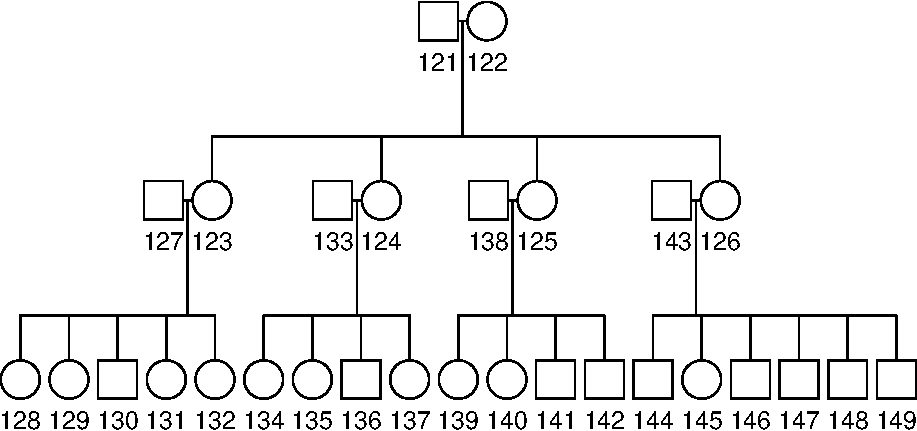
\includegraphics{familybasedpgms-example_files/figure-latex/unnamed-chunk-5-1.pdf}

\begin{verbatim}
#> Did not plot the following people: 150
\end{verbatim}

In this example, let's use the first replicate of the phenotypic data:

\begin{Shaded}
\begin{Highlighting}[]
\NormalTok{phen.df <-}\StringTok{ }\NormalTok{scen1}\OperatorTok{$}\NormalTok{phen.df[[}\DecValTok{1}\NormalTok{]]}
\end{Highlighting}
\end{Shaded}

The first rows of \texttt{phen.df} are shown in the following:

\begin{table}[!htbp] \centering 
  \caption{Phenotypes Dataset} 
  \label{} 
\begin{tabular}{@{\extracolsep{5pt}} cccc} 
\\[-1.8ex]\hline 
\hline \\[-1.8ex] 
 & X & Y & Z \\ 
\hline \\[-1.8ex] 
1 & $$-$1.686$ & $$-$1.452$ & $$-$1.101$ \\ 
2 & $0.919$ & $0.324$ & $0.788$ \\ 
3 & $$-$1.928$ & $$-$0.299$ & $$-$1.153$ \\ 
4 & $$-$0.957$ & $$-$0.308$ & $$-$0.085$ \\ 
5 & $$-$1.798$ & $0.546$ & $$-$0.101$ \\ 
6 & $1.040$ & $$-$0.148$ & $$-$0.310$ \\ 
\hline \\[-1.8ex] 
\end{tabular} 
\end{table}

Also, since no covariates was used in this simulation, let's define the
covariate dataset as NULL:

\begin{Shaded}
\begin{Highlighting}[]
\NormalTok{covs.df <-}\StringTok{ }\OtherTok{NULL}
\end{Highlighting}
\end{Shaded}

\subsection{Learning Total, Genetic, and Environmental Undirected
PGMs}\label{learning-total-genetic-and-environmental-undirected-pgms}

\begin{Shaded}
\begin{Highlighting}[]

\NormalTok{scenario =}\StringTok{ }\DecValTok{1}

\CommentTok{# Total number of individuals}
\NormalTok{N <-}\StringTok{ }\KeywordTok{sum}\NormalTok{(fam.nf) }

\CommentTok{# Here we are assuming that all individuals were sampled.}
\CommentTok{# Thus, the vector sampled is N-dimensional vector with all entries equal to 1.}
\CommentTok{# sampled <- rep(1, N) }

\KeywordTok{set.seed}\NormalTok{(}\DecValTok{12345}\NormalTok{)}
\NormalTok{sampled <-}\StringTok{ }\KeywordTok{sample}\NormalTok{(}\KeywordTok{c}\NormalTok{(}\OtherTok{TRUE}\NormalTok{, }\OtherTok{FALSE}\NormalTok{), }\DecValTok{900}\NormalTok{, }\DataTypeTok{replace=}\OtherTok{TRUE}\NormalTok{)}
\NormalTok{phen.df <-}\StringTok{ }\NormalTok{phen.df[sampled,]}
 
\NormalTok{fileID <-}\StringTok{ }\KeywordTok{paste0}\NormalTok{(}\StringTok{"scen"}\NormalTok{, scenario)}
\NormalTok{dirToSave <-}\StringTok{ }\KeywordTok{paste0}\NormalTok{(}\StringTok{"./objects-UDG-"}\NormalTok{, fileID, }\StringTok{"/"}\NormalTok{)}
\KeywordTok{dir.create}\NormalTok{(dirToSave, }\DataTypeTok{showWarnings=}\OtherTok{FALSE}\NormalTok{)}

\NormalTok{alpha =}\StringTok{ }\FloatTok{0.05}

\NormalTok{udgs.out <-}\StringTok{ }\KeywordTok{learnFamilyBasedUDGs}\NormalTok{(phen.df, covs.df, pedigrees, sampled, }
\NormalTok{                                 fileID, dirToSave, alpha, }\DataTypeTok{correction=}\OtherTok{NULL}\NormalTok{, }
                                 \DataTypeTok{max_cores=}\OtherTok{NULL}\NormalTok{, }\DataTypeTok{minK=}\DecValTok{10}\NormalTok{, }\DataTypeTok{maxFC =} \FloatTok{0.05}\NormalTok{,}
                                 \DataTypeTok{orthogonal=}\OtherTok{TRUE}\NormalTok{, }\DataTypeTok{useGPU=}\OtherTok{FALSE}\NormalTok{, }\DataTypeTok{debug=}\OtherTok{TRUE}\NormalTok{)}
\end{Highlighting}
\end{Shaded}

Now, we can check the learned undirected \emph{total} PGM.

Its adjacency matrix is:

\begin{Shaded}
\begin{Highlighting}[]
\NormalTok{udgs.out}\OperatorTok{$}\NormalTok{adjM}\OperatorTok{$}\NormalTok{t}
\CommentTok{#>   X Y Z}
\CommentTok{#> X 0 1 1}
\CommentTok{#> Y 1 0 1}
\CommentTok{#> Z 1 1 0}
\end{Highlighting}
\end{Shaded}

The estimates and p-values of the partial correlations are:

\begin{Shaded}
\begin{Highlighting}[]
\NormalTok{udgs.out}\OperatorTok{$}\NormalTok{pCor}\OperatorTok{$}\NormalTok{pCor_t}
\CommentTok{#> $estimates}
\CommentTok{#>            X          Y         Z}
\CommentTok{#> X         NA -0.4835768 0.6912148}
\CommentTok{#> Y -0.4835768         NA 0.7615219}
\CommentTok{#> Z  0.6912148  0.7615219        NA}
\CommentTok{#> }
\CommentTok{#> $pvalues}
\CommentTok{#>              X            Y            Z}
\CommentTok{#> X           NA 1.189697e-25 4.282081e-60}
\CommentTok{#> Y 1.189697e-25           NA 1.315617e-79}
\CommentTok{#> Z 4.282081e-60 1.315617e-79           NA}
\end{Highlighting}
\end{Shaded}

Plotting the learned PGM using its representation as an \texttt{igraph}
object:

\begin{Shaded}
\begin{Highlighting}[]
\CommentTok{# igraph object}
\NormalTok{udgs.out}\OperatorTok{$}\NormalTok{udg}\OperatorTok{$}\NormalTok{t}
\CommentTok{#> IGRAPH 4dcdbfb UN-- 3 3 -- }
\CommentTok{#> + attr: name (v/c)}
\CommentTok{#> + edges from 4dcdbfb (vertex names):}
\CommentTok{#> [1] X--Y X--Z Y--Z}

\KeywordTok{plot}\NormalTok{(udgs.out}\OperatorTok{$}\NormalTok{udg}\OperatorTok{$}\NormalTok{t, }\DataTypeTok{vertex.size=}\DecValTok{30}\NormalTok{, }
     \DataTypeTok{vertex.color=}\StringTok{"lightblue"}\NormalTok{)}
\end{Highlighting}
\end{Shaded}

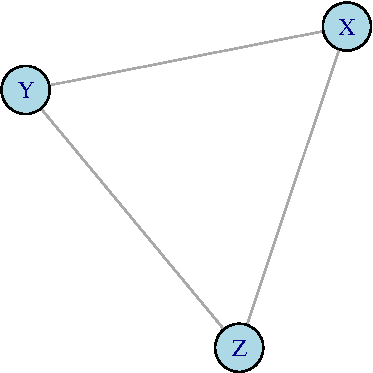
\includegraphics{familybasedpgms-example_files/figure-latex/unnamed-chunk-12-1.pdf}

Let's now check the learned undirected \emph{genetic} PGM.

Its adjacency matrix is:

\begin{Shaded}
\begin{Highlighting}[]
\NormalTok{udgs.out}\OperatorTok{$}\NormalTok{adjM}\OperatorTok{$}\NormalTok{g}
\CommentTok{#>   X Y Z}
\CommentTok{#> X 0 1 1}
\CommentTok{#> Y 1 0 1}
\CommentTok{#> Z 1 1 0}
\end{Highlighting}
\end{Shaded}

The estimates, p-values, and effective sizes of the partial correlations
are:

\begin{Shaded}
\begin{Highlighting}[]
\NormalTok{udgs.out}\OperatorTok{$}\NormalTok{pCor}\OperatorTok{$}\NormalTok{pCor_g}
\CommentTok{#> $estimates}
\CommentTok{#>            X          Y         Z}
\CommentTok{#> X         NA -0.5504830 0.7320944}
\CommentTok{#> Y -0.5504830         NA 0.7429468}
\CommentTok{#> Z  0.7320944  0.7429468        NA}
\CommentTok{#> }
\CommentTok{#> $pvalues}
\CommentTok{#>              X            Y            Z}
\CommentTok{#> X           NA 1.153901e-06 1.509676e-19}
\CommentTok{#> Y 1.153901e-06           NA 4.718409e-12}
\CommentTok{#> Z 1.509676e-19 4.718409e-12           NA}
\CommentTok{#> }
\CommentTok{#> $k}
\CommentTok{#>     X  Y   Z}
\CommentTok{#> X  NA 68 109}
\CommentTok{#> Y  68 NA  62}
\CommentTok{#> Z 109 62  NA}
\end{Highlighting}
\end{Shaded}

Plotting the learned PGM using its representation as an \texttt{igraph}
object:

\begin{Shaded}
\begin{Highlighting}[]
\CommentTok{# igraph object}
\NormalTok{udgs.out}\OperatorTok{$}\NormalTok{udg}\OperatorTok{$}\NormalTok{g}
\CommentTok{#> IGRAPH c163ddf UN-- 3 3 -- }
\CommentTok{#> + attr: name (v/c)}
\CommentTok{#> + edges from c163ddf (vertex names):}
\CommentTok{#> [1] X--Y X--Z Y--Z}

\KeywordTok{plot}\NormalTok{(udgs.out}\OperatorTok{$}\NormalTok{udg}\OperatorTok{$}\NormalTok{g, }\DataTypeTok{vertex.size=}\DecValTok{30}\NormalTok{, }
     \DataTypeTok{vertex.color=}\StringTok{"lightblue"}\NormalTok{)}
\end{Highlighting}
\end{Shaded}

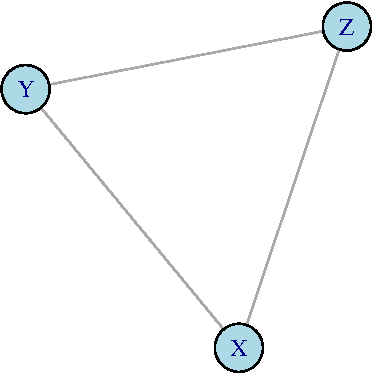
\includegraphics{familybasedpgms-example_files/figure-latex/unnamed-chunk-15-1.pdf}

Finally, let's check the learned undirected \emph{environmental} PGM.

Its adjacency matrix is:

\begin{Shaded}
\begin{Highlighting}[]
\NormalTok{udgs.out}\OperatorTok{$}\NormalTok{adjM}\OperatorTok{$}\NormalTok{e}
\CommentTok{#>   X Y Z}
\CommentTok{#> X 0 1 1}
\CommentTok{#> Y 1 0 1}
\CommentTok{#> Z 1 1 0}
\end{Highlighting}
\end{Shaded}

The estimates, p-values, and effective sizes of the partial correlations
are:

\begin{Shaded}
\begin{Highlighting}[]
\NormalTok{udgs.out}\OperatorTok{$}\NormalTok{pCor}\OperatorTok{$}\NormalTok{pCor_e}
\CommentTok{#> $estimates}
\CommentTok{#>            X          Y         Z}
\CommentTok{#> X         NA -0.4759565 0.6333600}
\CommentTok{#> Y -0.4759565         NA 0.7901565}
\CommentTok{#> Z  0.6333600  0.7901565        NA}
\CommentTok{#> }
\CommentTok{#> $pvalues}
\CommentTok{#>              X            Y            Z}
\CommentTok{#> X           NA 1.442939e-03 1.973361e-05}
\CommentTok{#> Y 1.442939e-03           NA 1.095614e-18}
\CommentTok{#> Z 1.973361e-05 1.095614e-18           NA}
\CommentTok{#> }
\CommentTok{#> $k}
\CommentTok{#>    X  Y  Z}
\CommentTok{#> X NA 42 38}
\CommentTok{#> Y 42 NA 82}
\CommentTok{#> Z 38 82 NA}
\end{Highlighting}
\end{Shaded}

Plotting the learned PGM using its representation as an \texttt{igraph}
object:

\begin{Shaded}
\begin{Highlighting}[]
\CommentTok{# igraph object}
\NormalTok{udgs.out}\OperatorTok{$}\NormalTok{udg}\OperatorTok{$}\NormalTok{e}
\CommentTok{#> IGRAPH cc8dd2a UN-- 3 3 -- }
\CommentTok{#> + attr: name (v/c)}
\CommentTok{#> + edges from cc8dd2a (vertex names):}
\CommentTok{#> [1] X--Y X--Z Y--Z}

\KeywordTok{plot}\NormalTok{(udgs.out}\OperatorTok{$}\NormalTok{udg}\OperatorTok{$}\NormalTok{e, }\DataTypeTok{vertex.size=}\DecValTok{30}\NormalTok{, }
     \DataTypeTok{vertex.color=}\StringTok{"lightblue"}\NormalTok{)}
\end{Highlighting}
\end{Shaded}

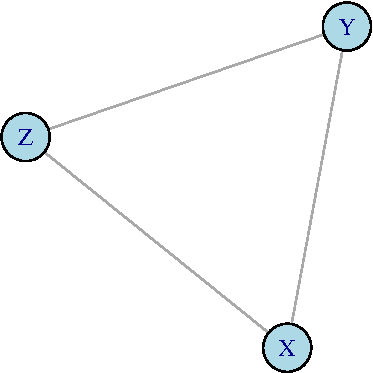
\includegraphics{familybasedpgms-example_files/figure-latex/unnamed-chunk-18-1.pdf}

\subsection{Learning Total, Genetic, and Environmental Directed Acyclic
PGMs}\label{learning-total-genetic-and-environmental-directed-acyclic-pgms}

\begin{Shaded}
\begin{Highlighting}[]
\NormalTok{fileID <-}\StringTok{ }\KeywordTok{paste0}\NormalTok{(}\StringTok{"scen"}\NormalTok{, scenario)}
\NormalTok{dirToSave <-}\StringTok{ }\KeywordTok{paste0}\NormalTok{(}\StringTok{"./objects-PC-"}\NormalTok{, fileID, }\StringTok{"/"}\NormalTok{)}
\KeywordTok{dir.create}\NormalTok{(dirToSave, }\DataTypeTok{showWarnings=}\OtherTok{FALSE}\NormalTok{)}

\NormalTok{alpha =}\StringTok{ }\FloatTok{0.05} \CommentTok{# significance level}

\NormalTok{dags <-}\StringTok{ }\KeywordTok{learnFamilyBasedDAGs}\NormalTok{(phen.df, covs.df, pedigrees, sampled,}
\NormalTok{   fileID, dirToSave, alpha, }\DataTypeTok{max_cores=}\OtherTok{NULL}\NormalTok{,}
   \DataTypeTok{minK=}\DecValTok{10}\NormalTok{, }\DataTypeTok{maxFC =} \FloatTok{0.05}\NormalTok{, }\DataTypeTok{orthogonal=}\OtherTok{TRUE}\NormalTok{, }\DataTypeTok{maj.rule=}\OtherTok{TRUE}\NormalTok{,}
   \DataTypeTok{useGPU=}\OtherTok{FALSE}\NormalTok{, }\DataTypeTok{debug=}\OtherTok{TRUE}\NormalTok{, }\DataTypeTok{savePlots=}\OtherTok{FALSE}\NormalTok{)}
\end{Highlighting}
\end{Shaded}

Now, we can check the learned directed acyclic \emph{total} PGM.

Its adjacency matrix is:

\begin{Shaded}
\begin{Highlighting}[]
\NormalTok{adjM_t <-}\StringTok{ }\KeywordTok{as}\NormalTok{(dags}\OperatorTok{$}\NormalTok{t, }\StringTok{"amat"}\NormalTok{)}
\NormalTok{adjM_t }
\CommentTok{#> Adjacency Matrix 'amat' (3 x 3) of type 'cpdag':}
\CommentTok{#>     X_t Y_t Z_t}
\CommentTok{#> X_t   .   .   .}
\CommentTok{#> Y_t   .   .   .}
\CommentTok{#> Z_t   1   1   .}
\end{Highlighting}
\end{Shaded}

Inspecting and plotting the learned PGM using its representation as an
\texttt{igraph} object:

\begin{Shaded}
\begin{Highlighting}[]
\CommentTok{# igraph object}
\NormalTok{dags}\OperatorTok{$}\NormalTok{t}
\CommentTok{#> Object of class 'pcAlgo', from Call:}
\CommentTok{#> pc(suffStat = suffStat, indepTest = familyBasedCITest, alpha = alpha, }
\CommentTok{#>     labels = paste0(colnames(phen.df), "_", type), skel.method = "stable", }
\CommentTok{#>     maj.rule = TRUE, solve.confl = TRUE, verbose = TRUE)}
\CommentTok{#> Number of undirected edges:  0 }
\CommentTok{#> Number of directed edges:    2 }
\CommentTok{#> Total number of edges:       2}

\NormalTok{pcalg}\OperatorTok{::}\KeywordTok{showEdgeList}\NormalTok{(dags}\OperatorTok{$}\NormalTok{t)}
\CommentTok{#> }
\CommentTok{#> Edge List: }
\CommentTok{#> }
\CommentTok{#> Undirected Edges:}
\CommentTok{#> }
\CommentTok{#> Directed Edges:}
\CommentTok{#>   X_t  -->  Z_t }
\CommentTok{#>   Y_t  -->  Z_t}

\NormalTok{igraph}\OperatorTok{::}\KeywordTok{plot.igraph}\NormalTok{(igraph}\OperatorTok{::}\KeywordTok{graph.adjacency}\NormalTok{(adjM_t), }
                    \DataTypeTok{vertex.size=}\DecValTok{30}\NormalTok{, }\DataTypeTok{vertex.color=}\StringTok{"lightblue"}\NormalTok{)}
\end{Highlighting}
\end{Shaded}

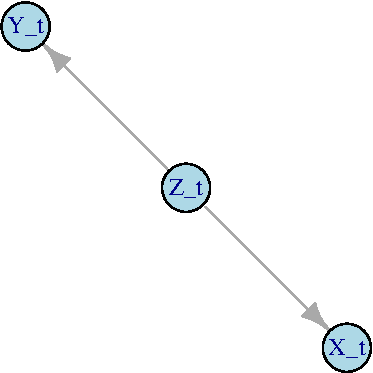
\includegraphics{familybasedpgms-example_files/figure-latex/unnamed-chunk-21-1.pdf}

Let's now check the learned directed acyclic \emph{genetic} PGM.

Its adjacency matrix is:

\begin{Shaded}
\begin{Highlighting}[]
\NormalTok{adjM_g <-}\StringTok{ }\KeywordTok{as}\NormalTok{(dags}\OperatorTok{$}\NormalTok{g, }\StringTok{"amat"}\NormalTok{)}
\NormalTok{adjM_g }
\CommentTok{#> Adjacency Matrix 'amat' (3 x 3) of type 'cpdag':}
\CommentTok{#>     X_g Y_g Z_g}
\CommentTok{#> X_g   .   .   .}
\CommentTok{#> Y_g   .   .   .}
\CommentTok{#> Z_g   1   1   .}
\end{Highlighting}
\end{Shaded}

Inspecting and plotting the learned PGM using its representation as an
\texttt{igraph} object:

\begin{Shaded}
\begin{Highlighting}[]
\CommentTok{# igraph object}
\NormalTok{dags}\OperatorTok{$}\NormalTok{g}
\CommentTok{#> Object of class 'pcAlgo', from Call:}
\CommentTok{#> pc(suffStat = suffStat, indepTest = familyBasedCITest, alpha = alpha, }
\CommentTok{#>     labels = paste0(colnames(phen.df), "_", type), skel.method = "stable", }
\CommentTok{#>     maj.rule = TRUE, solve.confl = TRUE, verbose = TRUE)}
\CommentTok{#> Number of undirected edges:  0 }
\CommentTok{#> Number of directed edges:    2 }
\CommentTok{#> Total number of edges:       2}

\NormalTok{pcalg}\OperatorTok{::}\KeywordTok{showEdgeList}\NormalTok{(dags}\OperatorTok{$}\NormalTok{g)}
\CommentTok{#> }
\CommentTok{#> Edge List: }
\CommentTok{#> }
\CommentTok{#> Undirected Edges:}
\CommentTok{#> }
\CommentTok{#> Directed Edges:}
\CommentTok{#>   X_g  -->  Z_g }
\CommentTok{#>   Y_g  -->  Z_g}

\NormalTok{igraph}\OperatorTok{::}\KeywordTok{plot.igraph}\NormalTok{(igraph}\OperatorTok{::}\KeywordTok{graph.adjacency}\NormalTok{(adjM_g), }\DataTypeTok{vertex.size=}\DecValTok{30}\NormalTok{, }\DataTypeTok{vertex.color=}\StringTok{"lightblue"}\NormalTok{)}
\end{Highlighting}
\end{Shaded}

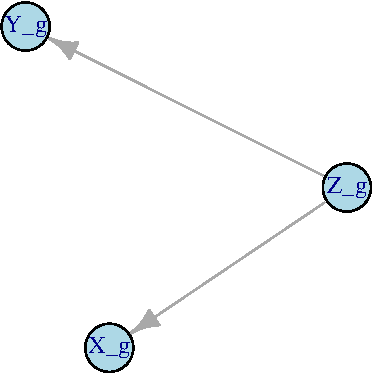
\includegraphics{familybasedpgms-example_files/figure-latex/unnamed-chunk-23-1.pdf}

Finally, let's check the learned directed acyclic \emph{environmental}
PGM.

Its adjacency matrix is:

\begin{Shaded}
\begin{Highlighting}[]
\NormalTok{adjM_e <-}\StringTok{ }\KeywordTok{as}\NormalTok{(dags}\OperatorTok{$}\NormalTok{e, }\StringTok{"amat"}\NormalTok{)}
\NormalTok{adjM_e }
\CommentTok{#> Adjacency Matrix 'amat' (3 x 3) of type 'cpdag':}
\CommentTok{#>     X_e Y_e Z_e}
\CommentTok{#> X_e   .   .   .}
\CommentTok{#> Y_e   .   .   .}
\CommentTok{#> Z_e   1   1   .}
\end{Highlighting}
\end{Shaded}

Inspecting and plotting the learned PGM using its representation as an
\texttt{igraph} object:

\begin{Shaded}
\begin{Highlighting}[]
\CommentTok{# igraph object}
\NormalTok{dags}\OperatorTok{$}\NormalTok{e}
\CommentTok{#> Object of class 'pcAlgo', from Call:}
\CommentTok{#> pc(suffStat = suffStat, indepTest = familyBasedCITest, alpha = alpha, }
\CommentTok{#>     labels = paste0(colnames(phen.df), "_", type), skel.method = "stable", }
\CommentTok{#>     maj.rule = TRUE, solve.confl = TRUE, verbose = TRUE)}
\CommentTok{#> Number of undirected edges:  0 }
\CommentTok{#> Number of directed edges:    2 }
\CommentTok{#> Total number of edges:       2}

\NormalTok{pcalg}\OperatorTok{::}\KeywordTok{showEdgeList}\NormalTok{(dags}\OperatorTok{$}\NormalTok{e)}
\CommentTok{#> }
\CommentTok{#> Edge List: }
\CommentTok{#> }
\CommentTok{#> Undirected Edges:}
\CommentTok{#> }
\CommentTok{#> Directed Edges:}
\CommentTok{#>   X_e  -->  Z_e }
\CommentTok{#>   Y_e  -->  Z_e}

\NormalTok{igraph}\OperatorTok{::}\KeywordTok{plot.igraph}\NormalTok{(igraph}\OperatorTok{::}\KeywordTok{graph.adjacency}\NormalTok{(adjM_e), }\DataTypeTok{vertex.size=}\DecValTok{30}\NormalTok{, }\DataTypeTok{vertex.color=}\StringTok{"lightblue"}\NormalTok{)}
\end{Highlighting}
\end{Shaded}

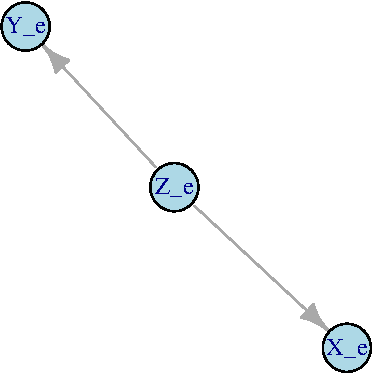
\includegraphics{familybasedpgms-example_files/figure-latex/unnamed-chunk-25-1.pdf}


\end{document}
